In this chapter we describe the structure of the H5 files used by
\progname to store the recorded data.

\begin{figure}
    \centering
    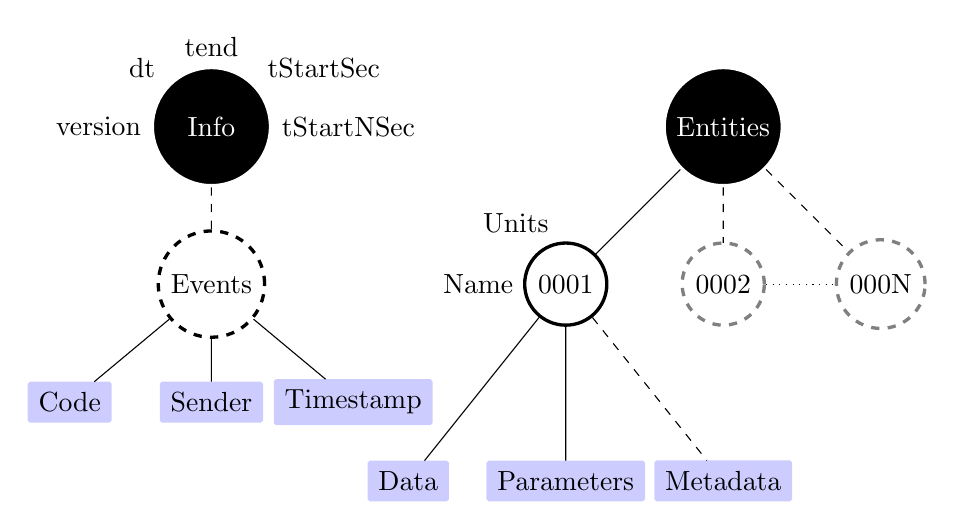
\begin{tikzpicture}[level distance=20mm,sibling distance=2cm,
        attr/.style={rectangle,draw,fill=black!20,rounded corners=.1ex, align=center},
        grp/.style={circle,draw=black,very thick,fill=white, align=center},    
        dataset/.style={rectangle,draw=blue!20,very thick,solid, fill=blue!20,rounded corners=.1ex, align=center}]


        \node[grp,
            white,right=0cm,fill=black, 
            minimum size=1.5cm,
            label=180:version,
            label=140:dt,
            label=90:tend,
            label=40:tStartSec,
            label=0:tStartNSec] (info) {Info}
        child {[sibling distance=18mm,level distance=15mm] node[grp] (events) {Events} 
            edge from parent[dashed]
            child { node[dataset] (ts) {Code} edge from parent[solid]}
            child { node[dataset] (ts) {Sender} edge from parent[solid]}
            child { node[dataset] (ts) {Timestamp} edge from parent[solid]}
        };

        \node[grp,right=6.5cm,white,fill=black,minimum size=1.5cm] (entities) {Entities}
            child {[sibling distance=20mm,level distance = 25mm] node[grp,label=180:Name,label=100:Units] (ent1) {0001} 
            child { node[dataset] (ts) {Data} edge from parent[solid]}
            child { node[dataset] (ts) {Parameters} edge from parent[solid]}
            child { node[dataset] (ts) {Metadata} edge from parent[dashed]}
            }
        child {[level distance = 20mm] node[grp,draw=gray] (ent2) {0002}
            edge from parent[dashed]} 
        child {[level distance = 20mm] node[grp,draw=gray] (entN) {000N} 
        edge from parent[dashed]};
    
        \draw [dotted] (ent2) -- (entN);
    \end{tikzpicture}
    \caption{Diagram of the data file model implemented with the H5Recorder.}
        \label{fig:hdf_diagram}
\end{figure}
